\section{Description and Methodology}

\subsection{Theoretical background}
Sound propagates through compressable and solid media as waves, and they are often described in terms of sinusoidal plane waves. The human ear can percept frequencies ranging from 20 Hz to 20,000 Hz, the higher frequency, the higher pitch.
\begin{figure}[h]
	\centering
	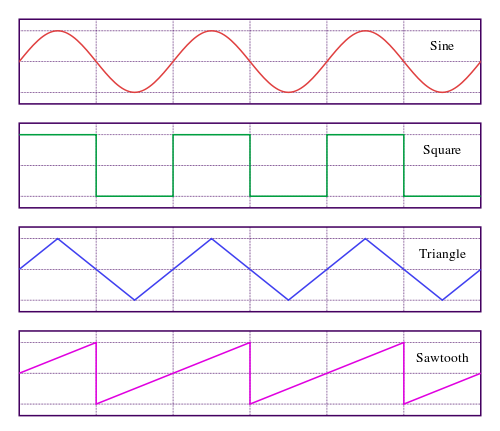
\includegraphics[width=8cm]{img/waveforms.png}
	\caption{Sine, square, triangle, and sawtooth waveforms. Figure found at \cite{wikipedia_sawtooth}.}
	\label{fig:sawtooth}
\end{figure}

In order to produce sound with the Digital-to-Analog converter, these waves need to be modeled. There are three simple ways: Square, triangle and sawtooth (see figure \ref{fig:sawtooth}). By repeatedly calculating the wave position(s) and write the result to the DAC, sound with the given frequency/frequencies are produced and can be percepted by the human ear if a headset is attached to the DAC. The more often write to the DAC, or the higher the sampling rate, the quality of the sound improves. \cite{compendium} states that a sampling rate of 48 kHz is a good reference value. 

\begin{figure}[h]
	\centering
	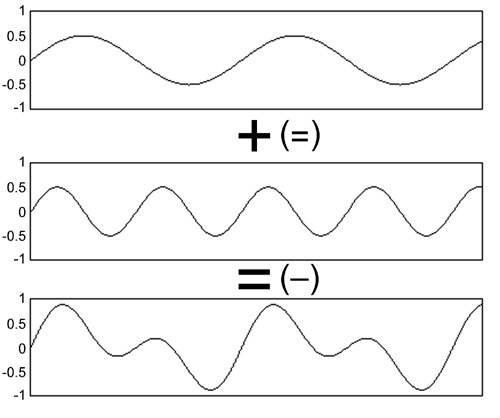
\includegraphics[width=8cm]{img/sumofsines.jpg}
	\caption{Adding sound waves together. Figure found at \cite{fourier}.}
	\label{fig:adding_waves}
\end{figure}
To play multiple frequencies together, you exploit the addititive nature of waves. You calculate each signal for a frequency independently, and then add them together (See figure \ref{fig:adding_waves}).

\subsection{Possible approaches}
We pictured two possible approaches to solve this exercise:

\begin{itemize}
	\item \textbf{Prestore the tracks in memory}: This requires us to generate the sample values that are to be written to the DAC before the program is started. The samples is then simply written to memory when the program starts. This solution requires a decent memory size. Since we got a total of 1024 bytes of flash storage, this solution enables us to store a total of 10 seconds of a track (48 000 samples per seconds and around 2 bytes per sample). Since we want to be able to play tracks that last longer then 10 seconds we did not choose this solution. The great advantage of this solution is that it is possibily the easiest way to utilitize the DMA, and let it handle all the transfers to the DAC. This completly frees the CPU to work on other tasks or go to sleep.
	\item \textbf{Calculate the sample values continuously}: Each time we get a timer interrupt we calculate the value to output to the DAC. This is requires more computations and is expected to consume more energy compared to just copy values from memory. The advantage of this solution is that we can play tracks of longer length and it is also easy to change what kind of signal we want to output. This is the solution we have chosen for this exercise.
	   
\end{itemize}

It is possible to make a hybrid of the two with the DMA. This way the DMA can copy sample values from a memory buffer to the DAC each time it is ready. When the memory buffer is empty, the DMA interrupts the CPU and the CPU fills up the buffer with new values. We figured that we wanted a running program wich functioned properly, rather then take the leap of faith with the chance of failure. The hybrid solution is probably more convenient than the first approach, and more energy efficient than the latter.  


\subsection{Project structure}
Here is a little overview of the files in the project. There will not be a thorough explanation of the code, as it is well documented. The project consist of two parts; the C code flashed to the \boardName\ (located in \emph{code/}) and a simple python script for generating samples from sheet music (located in \emph{sampler/}).

\begin{itemize}
	\item \emph{code/dac.c} - DAC initialization.
	\item \emph{code/ex2.c} - Contains the applications entry method. Sets up all pherepials and external modules. Will configure interrupt handling.
	\item \emph{code/gpio.c} - GPIO initialization.
	\item \emph{code/interrupt\_handlers.c} - Contains interrupt procedures for timers and GPIO. Will communicate with \emph{code/sampler.c} to set sampler modes and push samples onto the DAC.
	\item \emph{code/Makefile} - Makefile for cross compiling and uploading binaries to \boardName .
	\item \emph{code/sampler.c} - Independent module for sample calculation. Will generate sample values depending on the sampler mode.
	\item \emph{code/timer.c} - High and low frequency timer setup. Also contains logic for turning the low energy timer on and off.
	\item \emph{sampler/freq.csv} - Contains frequency values for all notes.
	\item \emph{sampler/Makefile} - Will generate and concatenate several tracks into one C source file which will be included in the data segment of the code uploaded to the board.
	\item \emph{sampler/sampler.py} - Python script for generating samples from sheet music.
\end{itemize}

Most of the C source files have a corresponding header to define their external interfaces.

\subsection{Setup}
Like last time, we initially developed a simple application with all the basics set up. The DAC, timer and GPIO was set up in the files dac.c, timer.c and gpio.c. The interrupts where handled in the interrupt\_handlers.c file. The main part of our program is the sampler.c. The interrupt handlers send and receive data to and from the sampler.c file. The GPIO handler set one of 9 modes in sampler.c and the timer interrupt handler pulls information from the sampler program and feeds it to the DAC.

\subsection{Sampler}
As explained, all logic for calculating DAC output is located in \emph{code/sampler.h}. This module requires some extra attention due to its importance. The external interface defines three functions:
\begin{itemize}
	\item \emph{sampler\_init()} - Initializes the sampler and loads the data structures with samples and initial values.
	\item \emph{sampler\_set\_mode(int mode)} - Interface for controlling the sampler behavior; that is changig waveforms and playing different sounds.
	\item \emph{sampler\_get()} - Will return a value between 0 and 2048, which is meant to be put directly on the DAC. The sampler has an internal constant named \emph{FREQUENCY}, which is the frequency \emph{sampler\_get} should be called. \emph{sampler\_get()} will return -1 if there are no tracks active.
\end{itemize}
\subsubsection{Sample file format}
\begin{figure}[h]
	\centering
	\begin{lstlisting}[language=C]
typedef struct sample {
	float hz;
	int ms;
} sample_t;
	\end{lstlisting}
	\caption{Sample struct}
	\label{file_format_struct}
\end{figure}
To be able to play sound sequences, we invented our own, very simple, audio format. It consists of simple structs, each contaning frequency and duration (see figure \ref{file_format_struct}) To represent a sequence, we placed several different samples in an array and kept track of the current index and elapsed time. The \emph{sampler\_get()}-function contains logic to call \emph{ms\_tick()} every millisecond, a function that decreases the current sample time left.\\
\\
To support multiple tracks, the one dimensional array containing samples was augmented to a two dimensional array. Also the variables containing the threshold and the remaining time for the current frequency was set to arrays. Now, all tracks would be updated every millisecound. To play different samples over each other, the different thresholds where scaled (so every track would contribute the same), added together and scaled once more before being sendt to the DAC.

\subsubsection{Setting track frequency and maintaining wave state}
Each track could independently have their frequencies set by the internal \emph{set\_hz()} function. When this function is invoked, it would alter two values; \emph{current\_height} and \emph{height\_threshold}. Together, these variables form a frequencys wave state. The \emph{height\_threshold} keeps the number of pulls (\emph{sampler\_get()} calls) between each wavetop, and \emph{current\_height} keeps the current position at the wave. At each pull, the \emph{current\_height} will be incremented by one and a new value for the current frequency can be calculated using the wave state variable set. All waveform functions (\emph{get\_sawtooth\_signal()}, \emph{get\_triangle\_signal()} and \emph{get\_square\_signal()}) are designed to operate with these variables.

\subsubsection{Enabling and disabling tracks}
In order to enable and disable tracks individually, a bitmap named \emph{active\_tracks} is used. On each pull, only tracks with their corresponding bit set to $1$ will be updated and contribute to the output. When this variable is updated using the \emph{set\_active} function, the sampler will also reset the sample indexes, making the tracks play audio from their starting position.

\subsubsection{Waveforms}
All tracks have their waves generated by the \emph{get\_signal()} function. This contains a switch on the \emph{waveform\_t} enum type, and returns the waveform as assigned in the global \emph{waveform} variable.


\subsection{Low energy timer and sleep modes}

To make our program more energy efficient, we made use of a low energy timer. This runs on a low frequency clock and, compared to the high frequency clock TIMER1 which have a frequency of 48 MHz, the low energy clock have a frequency of only 32 kHz. We expect that this timer should be more energy efficient.\\
\\
To enable the low energy timer, following steps have to be done:

\begin{enumerate}
	\item {Write 16 to CMU\_HFCORECLKEN0 to enable clock for low energy timers.}
	\item {Write 64 to CMU\_OSCENCMD to enable low energy oscilator LFRCO used by LFACLK. LFACLK is the clock used by LETIMER0. (See figure 11.1 in \cite{reference_manual})}
	\item {Write 4 to CMU\_LFACLKEN0 to enable the clock for the LETIMER0.}
	\item {Write 512 LETIMER0\_CTRL to set the top of the timer to the register COMP0. This makes it possible to use the LETimer as a regular timer. Since COMP0 is the top value, it will be reffered to as LETIMER0\_TOP.}
	\item {Write the the top value to LETIMER0\_TOP.}
	\item {Enable interrupts by writing 1 to LETIMER0\_IEN.}
	\item {Start the timer by writing 1 to LETIMER\_CMD.} 
\end{enumerate}

An interrupt is triggered each time the timer is done counting, which in our case means tick. When an interrupt is triggered the LETIMER0\_IRQHandler()-routine in \emph{interrupt\_handlers.c} is called. This pulls a value from the sampler and writes the correct output to the DAC. \\
\\
Little energy efficiency optimizations when playing the auido could be done, because of the many calculations that the CPU have to do on each timer interrupt. Utilitizing the low frequency timer was the most convenient solution to lowering the amperage.\\
\\
As we could not get the system to sleep while playing audio, we tried out a solution to get the micro controller down to Energy Mode 3 when idle. If we are done playing a track there is no need to output anything to the DAC. Therefore the sampler signals the interrupt-routine if we are done playing a sound by returning -1. The handler would then turn off the timer by calling stopLETimer()-routine in \emph{timer.c}. This turns off the low frequency clock LFACLK. With both the low and high frequency oscilators disabled, we end up in Energy Mode 3.
When a button is pressed, the sampler pontentially has been filled with data again so it signals the timer to start with the startLETimer()-routine in \emph{timer.c}. This turns on the low frequency clock LFACLK, and makes the sound system active again.
\\
The problem with this solution is that it does not scale. If any other low frequent peripheral is using the LFACLK, we need to most likely need to rewrite the timer start- and stop-routines. We would have to make the timer start and stops more specific, and write to the registers of the low energy timer instead. The highest energy mode we could enter, if we just turned off the timer and not the low frequency clock, would be EM2. Since we only use the low energy timer in this assignment, we stick with our first solution to the energy consumption problem. 
 



\subsection{Generating samples}
Our file format for the samples is really easy to deal with, as the only information you need to supply is the frequency and duration of the sample. However, we wanted to easier be able to play melodies in sheet music, so we made a python script simplifying this task for us. The python script accepts csv file format, which contains the following data:
\begin{itemize}
	\item Track name.
	\item Variable names.
	\item Beats per minute.
	\item List of note keys with corresponding length.
\end{itemize}

Please see the code for more details, and the corresponding Makefile to see how the script is used.

